%% LyX 2.3.4.2 created this file.  For more info, see http://www.lyx.org/.
%% Do not edit unless you really know what you are doing.
\documentclass[english,dvipsnames,aspectratio=169,handout]{beamer}
\usepackage{mathptmx}
\usepackage{algorithm2e}
\usepackage{eulervm}
\usepackage[T1]{fontenc}
\usepackage[latin9]{inputenc}
\usepackage{babel}
\usepackage{amstext}
\usepackage{amssymb}
\usepackage{graphicx}
\usepackage{ifthen}
\usepackage{xcolor}
\usepackage{xspace}
\usepackage{tikz}
\usetikzlibrary{tikzmark}
\usetikzlibrary{calc}
\usepackage{pgfplots}
%\pgfplotsset{compat=1.17}
\usepackage{booktabs}
\usepackage{xpatch}
\usepackage{multirow}
\usepackage{colortbl}
\usepackage{pgfpages}

%\setbeameroption{show notes on second screen}

\xpatchcmd{\itemize}
  {\def\makelabel}
  {\ifnum\@itemdepth=1\relax
     \setlength\itemsep{2ex}% separation for first level
   \else
     \ifnum\@itemdepth=2\relax
       \setlength\itemsep{1ex}% separation for second level
     \else
       \ifnum\@itemdepth=3\relax
         \setlength\itemsep{0.5ex}% separation for third level
   \fi\fi\fi\def\makelabel
  }
 {}
 {}

\ifx\hypersetup\undefined
  \AtBeginDocument{%
    \hypersetup{unicode=true,pdfusetitle,
 bookmarks=true,bookmarksnumbered=false,bookmarksopen=false,
 breaklinks=false,pdfborder={0 0 0},pdfborderstyle={},backref=false,colorlinks=true,
 allcolors=NYUPurple,urlcolor=LightPurple}
  }
\else
  \hypersetup{unicode=true,pdfusetitle,
 bookmarks=true,bookmarksnumbered=false,bookmarksopen=false,
 breaklinks=false,pdfborder={0 0 0},pdfborderstyle={},backref=false,colorlinks=true,
 allcolors=NYUPurple,urlcolor=LightPurple}
\fi

\makeatletter

%%%%%%%%%%%%%%%%%%%%%%%%%%%%%% LyX specific LaTeX commands.
%% Because html converters don't know tabularnewline
\providecommand{\tabularnewline}{\\}

%%%%%%%%%%%%%%%%%%%%%%%%%%%%%% Textclass specific LaTeX commands.
% this default might be overridden by plain title style
\newcommand\makebeamertitle{\frame{\maketitle}}%
% (ERT) argument for the TOC
\AtBeginDocument{%
  \let\origtableofcontents=\tableofcontents
  \def\tableofcontents{\@ifnextchar[{\origtableofcontents}{\gobbletableofcontents}}
  \def\gobbletableofcontents#1{\origtableofcontents}
}

%%%%%%%%%%%%%%%%%%%%%%%%%%%%%% User specified LaTeX commands.
\usetheme{CambridgeUS} 
\beamertemplatenavigationsymbolsempty


% Set Color ==============================
\definecolor{NYUPurple}{RGB}{87,6,140}
\definecolor{LightPurple}{RGB}{165,11,255}


\setbeamercolor{title}{fg=NYUPurple}
\setbeamercolor{frametitle}{fg=NYUPurple}

\setbeamercolor{background canvas}{fg=NYUPurple, bg=white}
\setbeamercolor{background}{fg=black, bg=NYUPurple}

\setbeamercolor{palette primary}{fg=black, bg=gray!30!white}
\setbeamercolor{palette secondary}{fg=black, bg=gray!20!white}
\setbeamercolor{palette tertiary}{fg=gray!20!white, bg=NYUPurple}

\setbeamertemplate{headline}{}
\setbeamerfont{itemize/enumerate body}{}
\setbeamerfont{itemize/enumerate subbody}{size=\normalsize}

\setbeamercolor{parttitle}{fg=NYUPurple}
\setbeamercolor{sectiontitle}{fg=NYUPurple}
\setbeamercolor{sectionname}{fg=NYUPurple}
\setbeamercolor{section page}{fg=NYUPurple}
%\setbeamercolor{description item}{fg=NYUPurple}
%\setbeamercolor{block title}{fg=NYUPurple}

\setbeamertemplate{blocks}[rounded][shadow=false]
\setbeamercolor{block body}{bg=normal text.bg!90!NYUPurple}
\setbeamercolor{block title}{bg=NYUPurple!30, fg=NYUPurple}



\AtBeginSection[]{
  \begin{frame}
  \vfill
  \centering
\setbeamercolor{section title}{fg=NYUPurple}
 \begin{beamercolorbox}[sep=8pt,center,shadow=true,rounded=true]{title}
    \usebeamerfont{title}\usebeamercolor[fg]{title}\insertsectionhead\par%
  \end{beamercolorbox}
  \vfill
  \end{frame}
}

\makeatother

\setlength{\parskip}{\medskipamount} 

\input ../macros

\begin{document}
\input ../rosenberg-macros

\title[DS-GA 1003]{Introduction to Structured Prediction}
\author{He He \\
Slides based on Lecture
\href{https://github.com/davidrosenberg/mlcourse/blob/gh-pages/Lectures/09.multiclass.pdf}{09} from David Rosenberg's course materials (\url{https://github.com/davidrosenberg/mlcourse})
}
\date{March 30, 2021}
\institute{CDS, NYU}

\makebeamertitle
\mode<article>{Just in article version}

\begin{frame}{Example: Part-of-speech (POS) Tagging}

\begin{itemize}
\item Given a sentence, give a part of speech tag for each word:
\end{itemize}
\begin{center}
\begin{tabular}{|c|c|c|c|c|}
\hline 
$x$ & $\underbrace{\mbox{[START]}}_{x_{0}}$ & $\underbrace{\mbox{He}}_{x_{1}}$ & $\underbrace{\mbox{eats}}_{x_{2}}$ & $\underbrace{\mbox{apples}}_{x_{3}}$\tabularnewline
\hline 
$y$ & $\underbrace{\mbox{[START]}}_{y_{0}}$ & $\underbrace{\mbox{Pronoun}}_{y_{1}}$ & $\underbrace{\mbox{Verb}}_{y_{2}}$ & $\underbrace{\mbox{Noun}}_{y_{3}}$\tabularnewline
\hline 
\end{tabular}
\par\end{center}

\pause{}
\begin{itemize}
\item $\cv=\left\{ \mbox{all English words}\right\} \cup\left\{ \mbox{[START]},"."\right\} $
\item $\cx=\cv^{n}$, $n=1,2,3,\ldots$ {[}Word sequences of any length{]}

\pause{}
\item $\cp=\left\{ \mbox{START},\mbox{Pronoun,Verb,Noun,Adjective}\right\} $
\item $\cy=\cp^{n},\,n=1,2,3,\ldots${[}Part of speech sequence of any length{]}

\end{itemize}
\end{frame}

\begin{frame}{Multiclass Hypothesis Space}

\begin{itemize}
\item \textcolor{blue}{Discrete} output space: $\cy(x)$ 
\begin{itemize}
\item Very large but has structure, e.g., linear chain (sequence labeling), tree (parsing)
\item Size depends on input $x$
\end{itemize}

\pause{}
\item Base Hypothesis Space: $\ch=\left\{ h:\cx\times\cy\to\reals\right\} $
\begin{itemize}
\item $h(x,y)$ gives \textcolor{blue}{compatibility score} between input $x$ and
output $y$ 
\end{itemize}

\pause{}
\item Multiclass hypothesis space
\[
\cf=\left\{ x\mapsto\argmax_{y\in\cy}h(x,y)\mid h\in\ch\right\} 
\]


\item Final prediction function is an $f\in\cf$. 
\item For each $f\in\cf$ there is an underlying compatibility score function
$h\in\ch$. 
\end{itemize}
\end{frame}
%

\begin{frame}{Structured Prediction}
\begin{itemize}
\item Part-of-speech tagging
\begin{table}
\begin{tabular}{llll}
$x\colon$ & he & eats & apples \\
$y\colon$ & pronoun & verb & noun 
\end{tabular}
\end{table}

\item Multiclass hypothesis space:
\begin{align}
& h(x,y) = w^T \Psi(x, y) \\
& \cf = \left\{ x\mapsto\argmax_{y\in\cy}h(x,y)\mid h\in\ch\right\}
\end{align}
\end{itemize}

\begin{itemize}
\item A special case of multiclass classification
\item  How to design the feature map $\Psi$? What are the considerations?
\note{contextual dependence, efficient argmax}
\end{itemize}
\end{frame}
%
\begin{frame}{Unary features}

\begin{itemize}
\item A  \textbf{unary feature} only depends on 
\begin{itemize}
\item the label at a \textcolor{blue}{single position}, $y_{i}$, and $x$ 
\end{itemize}

\item Example: 
\begin{eqnarray*}
\phi_{1}(x,y_{i}) & = & \ind{x_{i}=\mbox{runs}}\ind{y_{i}=\mbox{Verb}}\\
\phi_{2}(x,y_{i}) & = & \ind{x_{i}=\mbox{runs}}\ind{y_{i}=\mbox{Noun}}\\
\phi_{3}(x,y_{i}) & = & \ind{x_{i-1}=\mbox{He}}\ind{x_{i}=\mbox{runs}}\ind{y_{i}=\mbox{Verb}}
\end{eqnarray*}
 
\end{itemize}
\end{frame}
%
\begin{frame}{Markov features}

\begin{itemize}
\item A \textbf{markov feature} only depends on 
\begin{itemize}
\item two \textcolor{blue}{adjacent} labels, $y_{i-1}$ and $y_{i}$,
and $x$
\end{itemize}

\item Example: 
\begin{eqnarray*}
\theta_{1}(x,y_{i-1},y_{i}) & = & \ind{y_{i-1}=\mbox{Pronoun}}\ind{y_{i}=\mbox{Verb}}\\
\theta_{2}(x,y_{i-1},y_{i}) & = & \ind{y_{i-1}=\mbox{Pronoun}}\ind{y_{i}=\mbox{Noun}}
\end{eqnarray*}

\item Reminiscent of Markov models in the output space
\item Possible to have higher-order features 
 
\end{itemize}
\end{frame}
%
\begin{frame}{Local Feature Vector and Compatibility Score}
\begin{itemize}[<+->]
\item At each position $i$ in sequence, define the \textbf{local feature
vector} (\textcolor{blue}{unary} and \textcolor{red}{markov}):
\begin{eqnarray*}
\Psi_{i}(x,y_{i-1},y_{i}) & = & (\phi_{1}(x,{\color{blue}y_{i}}),\phi_{2}(x,{\color{blue}y_{i}}),\ldots,\\
 &  & \theta_{1}(x,{\color{red}y_{i-1},y_{i}}),\theta_{2}(x,{\color{red}y_{i-1},y_{i}}),\ldots)
\end{eqnarray*}

\item And \textbf{local compatibility score} at position $i$:
$\left\langle w,\Psi_{i}(x,y_{i-1},y_{i})\right\rangle $. 

\item The compatibility score for $\left(x,y\right)$
is the sum of local compatibility scores: 
\begin{align}
\sum_{i}\left\langle w,\Psi_{i}(x,y_{i-1},y_{i})\right\rangle 
= \left\langle w,\sum_{i}\Psi_{i}(x,y_{i-1},y_{i})\right\rangle
= \left\langle w,\Psi(x,y)\right\rangle ,
\end{align}
where we define the \textbf{sequence feature vector} by 
\[
\Psi(x,y)=\sum_{i}\Psi_{i}(x,y_{i-1},y_{i}). \qquad \text{\color{blue}decomposable}
\]
\end{itemize}
\end{frame}

\begin{frame}
{Structured perceptron}
\begin{algorithm}[H]
	Given a dataset $\sD=\pc{(x, y)}$\;
	Initialize $w\leftarrow 0$\;
	\For{$\text{iter} = 1,2,\ldots,T$}
	{
	\For{$(x,y) \in \sD$}
 	{
 		$\hat{y} = \argmax_{y'\in{\color<2->{red}\sY(x)}} w^T\psi(x, y')$\;
 		\If(\tcp*[h]{We've made a mistake}){$\hat{y} \neq y$}{ 
 		$w \leftarrow w + \Psi(x, y)$ \tcp*[l]{Move the scorer towards $\psi(x, y)$}
 		$w \leftarrow w - \Psi(x, \hat{y})$ \tcp*[l]{Move the scorer away from $\psi(x, \hat{y})$}
 		}
  	}
  	}
\end{algorithm}
\onslide<2->{
Identical to the multiclass perceptron algorithm except the $\argmax$ is now over the structured output space $\sY(x)$.
}
\end{frame}
%

\begin{frame}
{Structured hinge loss}
\begin{itemize}
\item Recall the generalized hinge loss
\begin{align}
\ell_\text{hinge}(y, \hat{y}) \eqdef
\max_{y'\in{\color{blue}\sY(x)}}\p{
\Delta(y, {y'}) +
\left\langle w, \p{\Psi(x, {y'}) - \Psi(x, {y}}) \right\rangle
}
\end{align}

\item What is $\Delta(y, {y'})$ for two sequences?
\pause
\item \textbf{Hamming loss} is common:
\[
\Delta(y,y')=\frac{1}{L}\sum_{i=1}^{L}\ind{y_{i}\neq y_{i}'}
\]
where $L$ is the sequence length.

\item Can generalize to the cost-sensitive version using $\delta(y_{i},y_{i}')$

\end{itemize}
\end{frame}

\begin{frame}
{Structured SVM}
\textcolor{Green}{Exercise}:
\begin{itemize}
\item Write down the objective of structured SVM using the structured hinge loss.
\item Stochastic sub-gradient descent for structured SVM (similar to HW3 P3)
\item Compare with the structured perceptron algorithm
\end{itemize}
\end{frame}


\begin{frame}
{The argmax problem for sequences}
\pause
\begin{description}[<+->]
\item[Problem]
To compute predictions, we need to find 
$\argmax_{y\in\cy(x)}\left\langle w,\Psi(x,y)\right\rangle$, and $\left|\cy(x)\right|$ is \textcolor{blue}{exponentially} large.

\item[Observation]
$\Psi(x,y)$ decomposes to $\sum_i \Psi_i(x,y)$.

\item[Solution]
Dynamic programming (similar to the Viterbi algorithm)
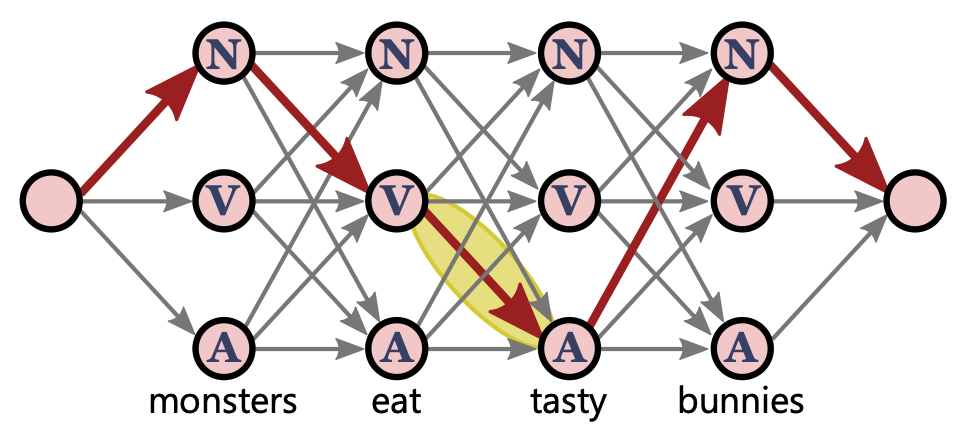
\includegraphics[height=0.4\textheight]{figures/dp}
What's the running time?
\note<.>{Let $K=\vert\sY\vert$, DP runtime $O(K^2L)$, $m$th order Markov feature has runtime $O(K^mL)$, naive runtime $O(K^L)$.}
\end{description}
\let\thefootnote\relax\footnotetext{\tiny{Figure by Daum\'e III. A course in machine learning. Figure 17.1}.}
\end{frame}

\begin{frame}
{The argmax problem in general}
Efficient problem-specific algorithms:
\begin{table}
\begin{tabular}{llll}
\toprule
problem & structure & algorithm \\
\midrule
constituent parsing & binary trees with context-free features & CYK  \\
dependency parsing & spanning trees with edge features & Chu-Liu-Edmonds \\
image segmentation & 2d with adjacent-pixel features & graph cuts \\
\bottomrule
\end{tabular}
\end{table}
\pause

General algorithm:
\begin{itemize}
\item Integer linear programming (ILP)
\begin{align}
\max_z\; a^Tz \quad \text{s.t. linear constraints on $z$}
\end{align}
\item $z$: indicator of substructures, \eg $\1\pc{y_i=\text{article and }y_{i+1}=\text{noun}}$
\item constraints: $z$ must correspond to a valid structure
\end{itemize}
\end{frame}

\begin{frame}
{Conclusion}
Multiclass algorithms
\begin{itemize}
\item Reduce to binary classification, \eg OvA, AvA, ECCO
\begin{itemize}
\item Good enough for simple multiclass problems
\end{itemize}
\item Generalize binary classification algorithms using multiclass loss
\begin{itemize}
\item Useful for problems with extremely large output space, \eg structured prediction
\item Related problems: ranking, multi-label classification
\end{itemize}
\end{itemize}
\end{frame}

\end{document}
